\section{Design}

CLAS12 Trigger System is designed as 3-stage pipeline-style system with total latency up to 8us. Stage 1 receives information from various CLAS12 detecrors and performs data processing in according to the type of detector. Stage 2 performs timing and geometry coincidence between different subset of dectors in 6 groups in according to 6-sector CLAS12 detector structure, as well as coincidence with information from central detectors. Stage 3 forms final trigger decision.
CLAS12 Trigger diagram is shown on Fig.~\ref{fig:TriggerDiagram}.

\begin{figure}[hbt]
	\centering
	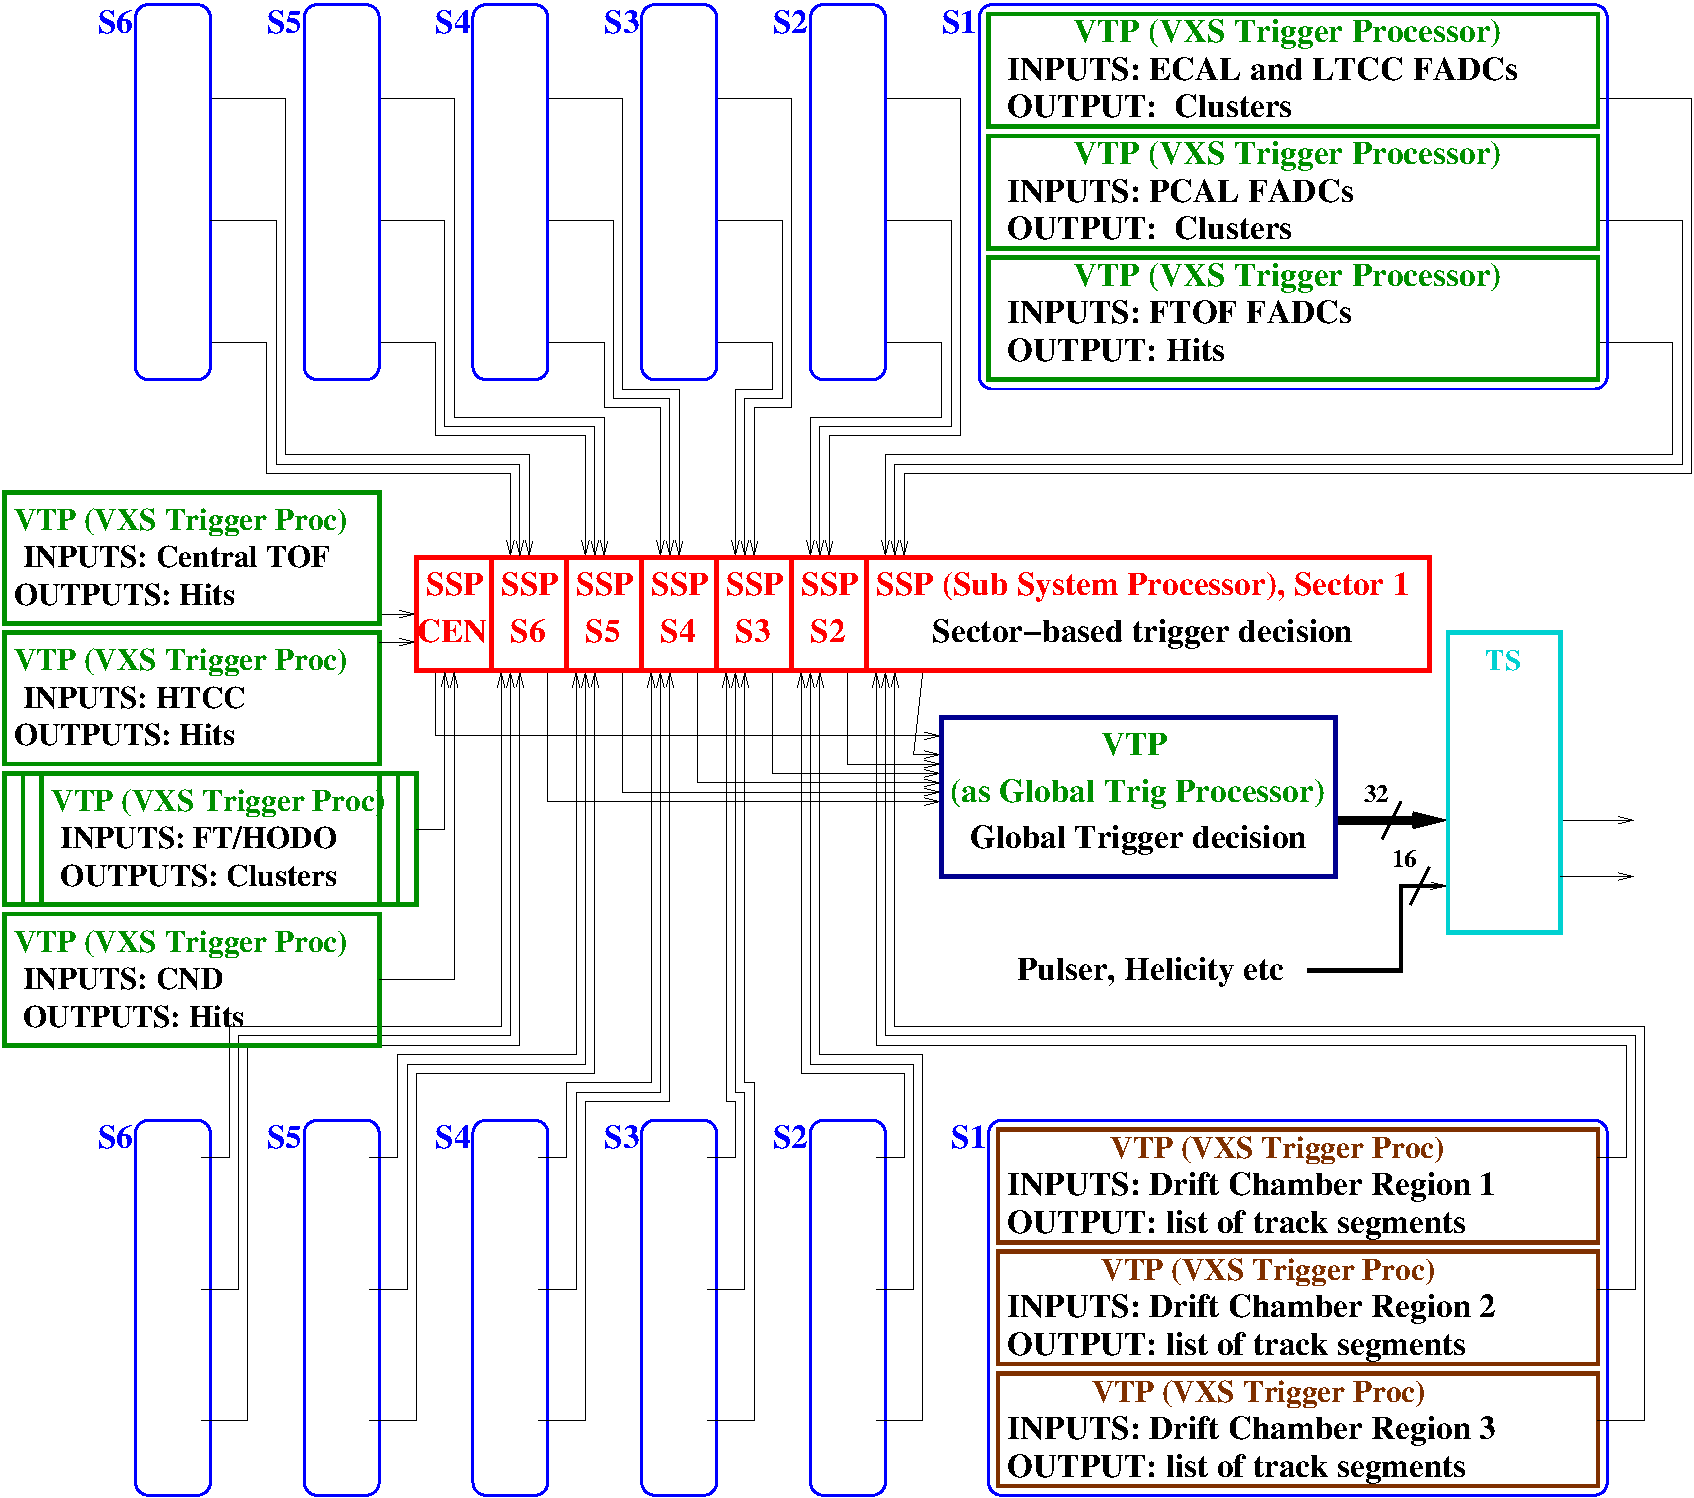
\includegraphics[width=1.0\columnwidth,keepaspectratio]{img/CLAS12_TRIGGER_1.pdf}
	\caption{CLAS12 Trigger System Diagram}
	\label{fig:TtiggerDiagram}
\end{figure}


\subsection{Stage 1} The most complex processing is performed for electromagnetic calorimeters (cluster finding) and drift chamber tracker (segment and road finding). In following sections we'll describe various trigger components design.

\subsubsection{FADCs as initial trigger information}

Almost all photomultiplier-based detectors in CLAS12 uses JLAB VXS 250Mhz Flash ADCs as starting point of the trigger logic (ref). Every channel of those FADC boards are pre-programmed with gain, pedestal and amplitude threshold above pedestal. Every pulse above amplitude threshold is integrated and sent to the corresponding section of the Stage 1 trigger logic. 16-channel FADC boards are reporting 13-bit pulse integrals and 3-bit pulse time every 32 ns, allowing following trigger logic to restore 4 ns pulse resolution while double pulse resolution remains 32 ns. Based on FADC reporting schedule following trigger logic stages can work on 250MHz clock, athought in that case we found it hard to meet FPGA timing, and our Stage 1 algorithms are running on 125MHz or slowers clocks as described below.

\subsubsection{DCRBs as trigger information}

Drift chamber-based trigger is using JLAB 125Mhz DCRB Discriminator/TDC boards to feed trigger system. Those 96-channel units reporting hits above pre-programmed thresholds every 16 ns.

\subsubsection{Electromagnetic calorimeters} sergey

CLAS12 two electromagnetic calorimeters (ref) consists of multiple layers of scintillating strips and lead sheets with photomultipliers readout on one side of scintillators (Fig.). Primary goal of those detectors is electron identification by defining energy and coordinate of the electromagnetic showers, called clusters. Cluster finding algorithm was well established during offline data processing development, and was adopted for trigger implementation with some simplifications.

First, it searches for one-dimensional clusters in each of three views, sorting them by energy and keeping only those above threshold, but not more then four. Second, it searches for two-dimensional clusters looking for crosses between three views. For two-dimension clusters found, it performs attenuation correction based on pre-loaded attenuantion length of the scintillation strips and distance from cluster to PMT, and correct cluster energy. Finally, it sorts two-dimension clusters by energy and report those above threshold, but not more then four. For every cluster, energy and coordinates are reported to the Stage 2 every 8 ns. There is an persistency parameter allowing to report the same clusters for several consequative 8 ns intervals to ensure timing coincidence with another trigger components, as well as timing delay parameter for the same purpose.

It should be mentioned that such algorithm is designed to found clusters with maximum energy targeting electrons identification. For some CLAS12 experiments, it was necessary to identify minimum-ionizing particles (MIPs) using the same trigger component. For that purpose, clusters with energy below certain threshold were selected. Such method works for events where the number of clusters does not exceed four, otherwise there is a risk of loosing low-energy clusters corresponding to MIPs. Intensive trigger efficiency studies were conducted for such cases, and MIP trigger efficiency was measured and found acceptable.


\subsubsection{Drift Chamber} sergey,ben

CLAS12 Drift Chamber (ref) contains six superlayers, six layers in each superlayers, 112 wires in every layer. Trigger algorithm was designed as two-step process.

First it searches for segments in each of six superlayers, reporting 112-bit mask with bits set for segments found. Search for segments is conducted based on pre-loaded segment dictionary, generated by drift chamber simulation software based on internal superlayer wires location. In case if several segments found in the same location the one with maximum number of hits are kept. In theory the number of hit wires in one segment can vary from 6 to 12 depending on track position and angle. On practice, the number of hits can be less because of drift chamber inefficiencies and broken wires, so threshold for segment finder in trigger logic was set to 4 and sometimes to 3.

After segment search complete and six 112-bit masks are ready second step is performed. On that step pre-loaded road dictionary is used to identify possible track candidates (so-called road finding). At least five out of six superlayers are required to satisfy trigger condition. All found roads are reported to the Stage 2 every 16 ns. Reported information contains ... for geometry match on Stage 2.



\subsubsection{High Threshold Cherenkov Counter} sergey

CLAS12 High Threshold Cherenkov Counter (HTCC, ref) detects electrons and serves as one of primary elements of electron trigger logic. It consists of 48 sections readout by PMTs connected to FADCs (Fig.~\ref{fig:multihitHTCC}). For trigger purposes 2x2 section sliding window is used to identify clusters. Configuration parameters includes single channel energy threshold, cluster multiplicity threshold and cluster energy threshold. Resilts are reported to Stage 2 as 48-bit masks every 4 ns.


\subsubsection{Forward Time-Of-Flight Counter} sergey

CLAS12 Forward Time-Of-Flight Counter (FTOF, ref) contains several layers of scintillating slabs, but only one layer is used by trigger logic. It contains 64 counters with PMT readout from both ends. When both end PMTs reports signal trigger system consider it as hit. 64-bit hit mask reported to the Stage 2 every 4 ns. Trigger logic configuration includes single channel energy threshold and threshold for SQRT(EleftxEright). FTOF participates in non-electron triggers such as muon trigger.


\subsubsection{Central Time-Of-Flight Counter} sergey

CLAS12 Central Time-Of-Flight Counter (CTOF, ref) consists of 48 scintillation slabs, surrounding target as barrel, with PMT readout from both ends. Its trigger logic is similar to FTOF one, with 48-bit mask reported every 4 ns.


\subsubsection{Neutron Detector} sergey

CLAS12 Neutron Detector (CND, ref) consists of three layers of scintillation slabs, installed behind CTOF, with 24 slabs per layer and 72 counters total. Its trigger logic is similar to FTOF/CTOF one, with 24-bit mask reported every 4 ns (usually inner layer only).


\subsubsection{Forward Calorimeter and Hodoscope} andrea,ben


\subsection{Stage 2} ben


\subsection{Stage 3} ben

